\chapter{Literature Review}

\section{Evolution of Object Detection}
The transition from feature engineering (Viola \& Jones, 2001) to deep learning (YOLO) has revolutionized detection, though general models often fail in clinical scenes (Diop et al., 2025).

\section{Pediatric Anthropometry}
Infant anatomy (1/4 ratio) differs significantly from adults (1/7.5 ratio), necessitating scale-invariant modeling (Mlinarić et al., 2024; Lin et al., 2022).

\section{Handling Occlusion in Ghanaian OPDs}
The ``Invisible Child'' phenomenon is a documented failure point in standard NMS algorithms (Addotey-Delove et al., 2023).

\section{Specialized Pediatric Datasets}
The Child Detection Dataset (CDD) provides real-world clinical benchmarks for fine-tuning.
\begin{figure}[h]
    \centering
    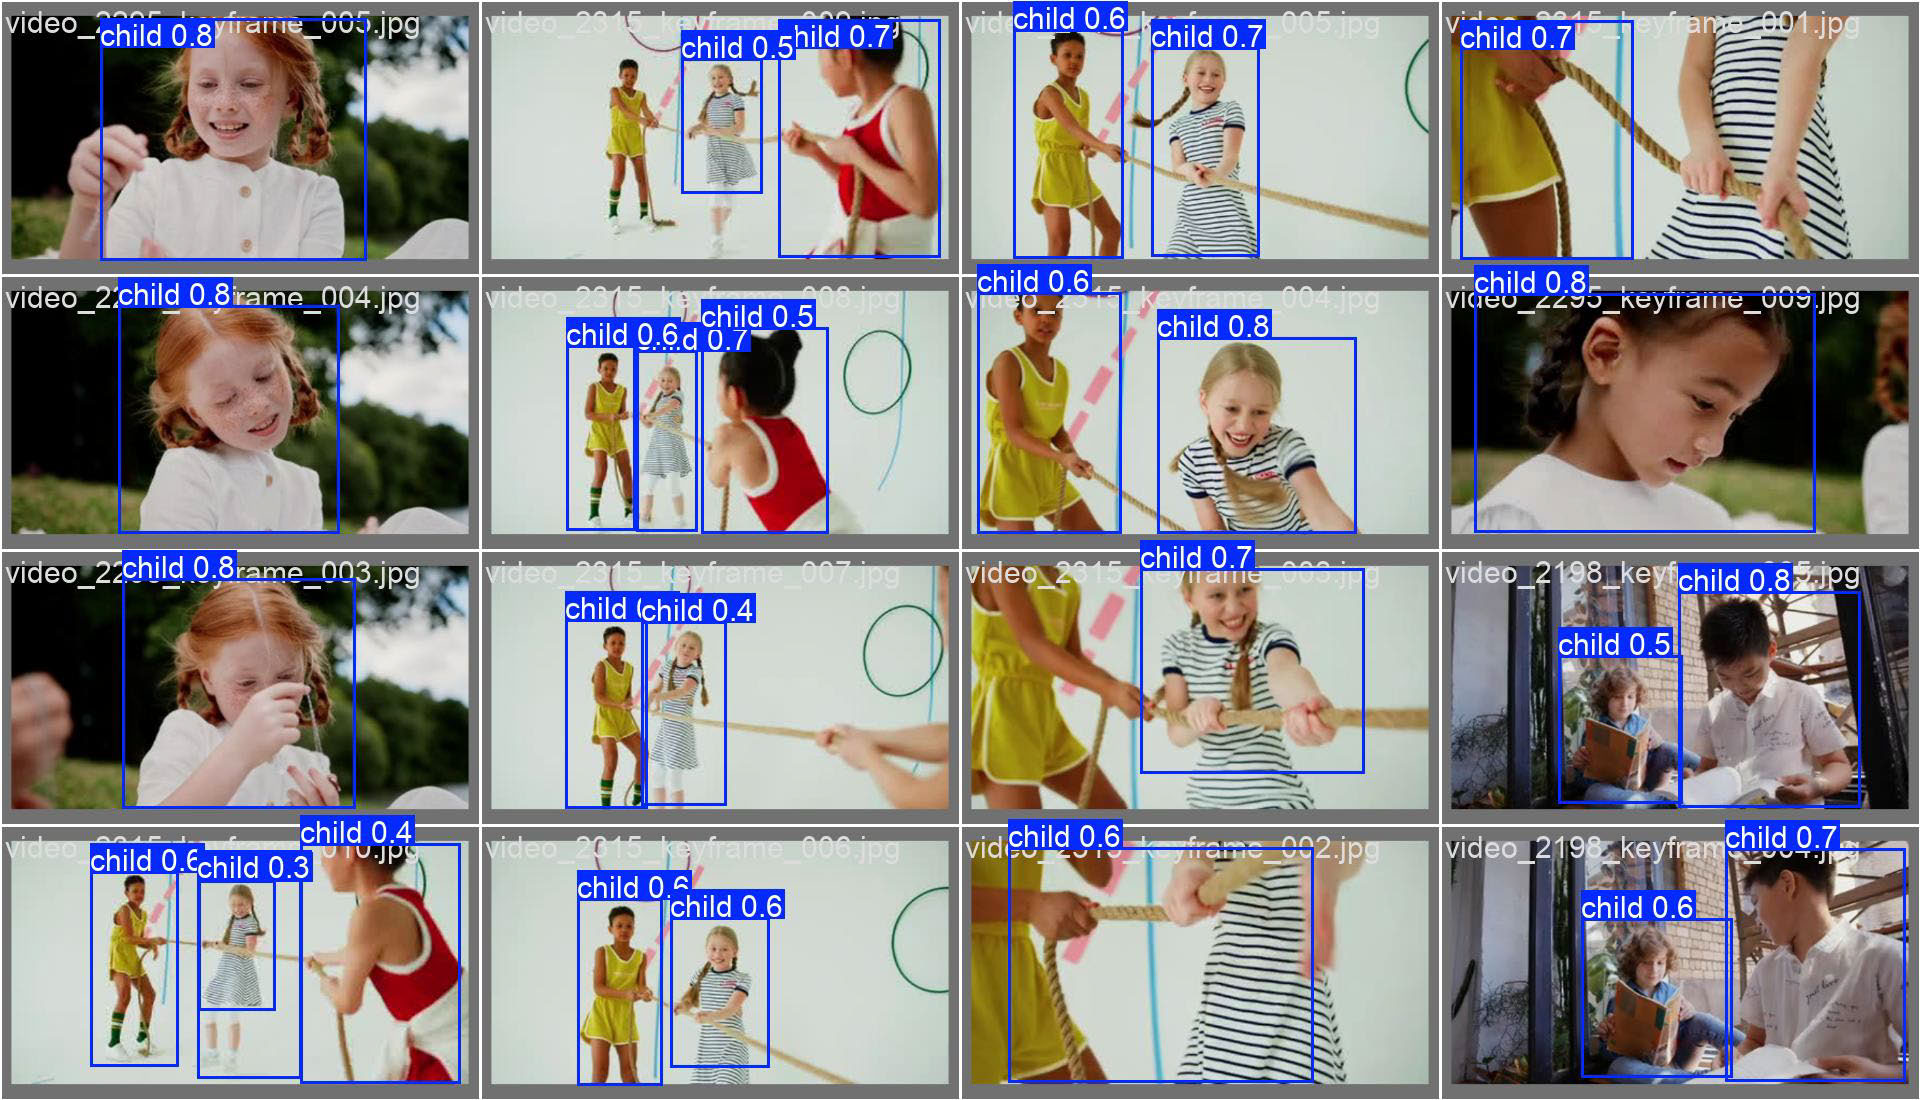
\includegraphics[width=0.8\textwidth]{images/fig-008.jpg}
    \caption{Sample results from the Child Detection Dataset (CDD) illustrating diverse pediatric postures and interactions.}
    \label{fig:cdd_samples}
\end{figure}

\section{Clinical Monitoring and Accuracy}
High-precision tracking is critical for infantile spasm detection and NICU monitoring (Diop et al., 2024; Keles \& Bagci, 2023).
\begin{figure}[h]
    \centering
    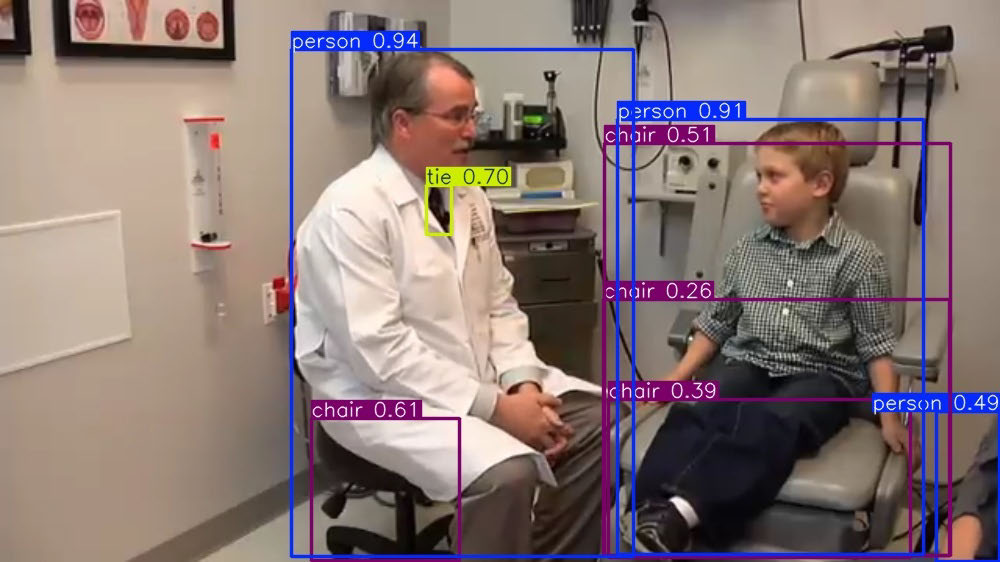
\includegraphics[width=0.8\textwidth]{images/fig-010.jpg}
    \caption{Comparative analysis: General YOLO limitations (left) versus specialized pediatric fine-tuning (right) in a clinical consultation scene.}
    \label{fig:yolo_comp}
\end{figure}
